% !TeX root = report.tex
% !TeX encoding = UTF-8
% !TeX spellcheck = en_US
% !TeX document-id = {b18791db-4bf7-45f4-b2cb-865b91539759}
%
% Report for Student Intervention System
% Udacity MLND Project 2
%
% Aravind Battaje

\documentclass{article}

% Packages used
\usepackage[margin=1in]{geometry}
\usepackage{multirow}
\usepackage{booktabs}
\usepackage{graphicx}
\usepackage{caption}
\usepackage{subcaption}
\usepackage{amsmath}

% Begin document
\begin{document}
	
	\title{Project Report: Student Intervention System}
	\author{Aravind Battaje}
	\maketitle
	
	\section{Project Steps}
	The goal of the project is to find a suitable supervised machine learning algorithm that can identify students who might need early intervention, by predicting their success/failure in graduation from the current records. To accomplish this task, three supervised learning models are probed for their suitability, and the best of them is later fine-tuned to get the best possible learning algorithm. All the three models are realized with the help of \texttt{scikit-learn}. For each of three models, a preliminary analysis is performed about its suitable basic configuration, costs and performance. Because of the small size of the dataset, cost and performance are measured by running multiple trials on shuffled data. The overall best performer that balances cost and performance is then fine-tuned using grid search (on parameters) and final predictions are made.
	
	\section{Classification vs Regression}
	A machine learning algorithm can be classified into two types, based on its nature of outputs, viz., classification and regression. Classification supports outputs of discrete values and regression outputs continuous values. This project entails a classification type of problem because the output desired from the \emph{intervention system} is discrete in nature, i.e., a student graduates or not from his/her current characteristics. Regression would be more suitable for, say an algorithm that predicts the final exam score from a student's current academic records.
	
	\section{Dataset}
	Several qualities of students such as their family background, social characteristics, extra-curricular activities, etc., along with the information if they graduated or not, are given along with the project in \texttt{student-data.csv}. The dataset possesses following characteristics:
	\begin{center}
		\begin{tabular}{c|c}
			\toprule
			Total number of students & 395 \\
			Number of students who passed & 265 \\
			Number of students who failed & 130  \\
			Graduation rate of the class & 67.09\% \\
			Number of features of dataset & 30 \\
			\bottomrule
		\end{tabular}
		\label{tab:data_characteristics}
	\end{center}
	
	\section{Training and Evaluating Models}
	Three supervised learning algorithms from \texttt{scikit-learn} were probed for their potential in \emph{best} modeling the student intervention problem. 
	\subsection{Naive Bayes Classifier}
	Naive Bayes Classifier is one of the simplest, and yet powerful algorithms used in supervised learning. It is a subset of the more complex generalization - Bayesian inference - in that, the likelihood of a hypothesis for modeling the data is inferred from the likelihood of data given a hypothesis. An (contrived) example which uses some of the features of the data provided in this project (\texttt{student-data.csv}) illustrates a few basic principles. Figure \ref{fig:belief_bayesian_inference} shows a belief network modeled with the classification variable \emph{passed} dependent on three features, with a certain conditionality evident between them. From the data (training), conditional probabity tables for each node is calculated, and so when a new data sample (testing) is introduced, the joint probability for \emph{passed} is calculated by simply multiplying relevant entries from the table. That is, assuming $v_1$, $v_2$ and $v_3$ represent the variables from the sample for \emph{goout}, \emph{freetime} and \emph{failures} respectively, 
	\[P(passed=1, goout=v_1, freetime=v_2, failures=v_3)\] will give the probabilty of student passing. This joint probability can be expressed as, \[P(...) = \prod_{i=1}^{n}P(v_i|Parents(Y_i)),\] where $P(passed=1)$, $P(goout=v_1|passed=1)$, $P(freetime=v_2|passed=1)$ and $P(failures=v_3|freetime=v_2,goout=v_1)$ will be the individual terms, derived from the belief network.
	
	\begin{figure}[h]
		\centering
		\begin{subfigure}[h]{0.4\textwidth}
			\centering
			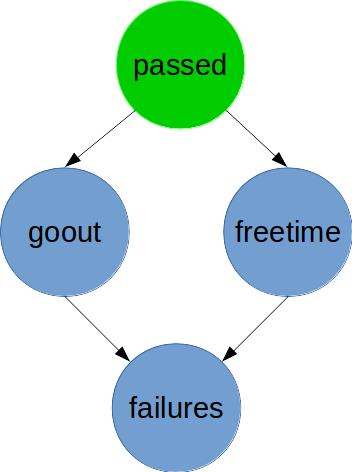
\includegraphics[scale=0.4]{example_belief_network_full}
			\caption{Bayesian Inference}
			\label{fig:belief_bayesian_inference}
		\end{subfigure}
		\begin{subfigure}[h]{0.4\textwidth}
			\centering
			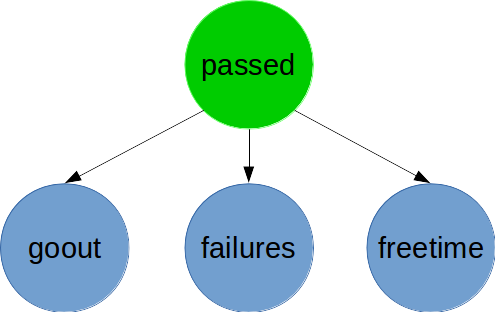
\includegraphics[scale=0.4]{example_belief_network_naive}
			\caption{Naive Bayes}
			\label{fig:belief_naive_bayes}
		\end{subfigure}
		\caption{Example belief networks with some of the features of \texttt{student-data}. \emph{passed} is the classification variable indicating if a student will pass or not; \emph{goout} indicates the time spent by a student going out with friends; \emph{freetime} indicates the free time a student gets after school; and, \emph{failures} indicates a student's failures in the past.}
	\end{figure}
	
	Naive Bayes Classifier shown in Figure \ref{fig:belief_naive_bayes} on the other hand assumes conditional independence between the features, and models the classification variables as being directly dependent on all features. The joint probability $P(passed=1, goout=v_1, freetime=v_2, failures=v_3)$ thus is much simpler: \[P(...) = P(passed=1)P(goout=v_1|passed=1)P(freetime=v_2|passed=1)P(failures=v_3|passed=1)\] 
	Computationally this is cheaper than the more complicated belief network of Figure \ref{fig:belief_bayesian_inference}, but more importantly, the computational cost of finding the best arrangement of nodes in the belief network during training grows exponentially with number of nodes (or features). Therefore, Bayesian inference - ideally considered as the \emph{gold} standard for supervised learning - becomes impractical. Nevertheless, Naive Bayes still stands out pretty well even as it assumes no causality between the several features of the data - it works surprisingly well in many applications, for instance in spam-filtering and such text-based classifiers \cite{Metsis06}. Although the dataset size provided with the project is small, and almost all learning algorithm is suscpetible to the \emph{curse of dimensionality}, Naive Bayes Classifier is extremely efficient and is worthy of setting a benchmark for other algorithms to compete against.

	\begin{table}[h]
		\centering
		\begin{tabular}{l|ccc}
			\toprule
			{} & \multicolumn{3}{c}{Training set size} \\
			{} &       100 &       200 &       300 \\
			\midrule
			Training time (msec)                  &  1.136737 &  1.401565 &  1.677573 \\
			Prediction time - Training set (msec) &  0.539596 &  0.743282 &  0.940869 \\
			Prediction time - Testing set (msec)  &  0.535090 &  0.538042 &  0.541995 \\
			F1 score - Training set               &  0.703436 &  0.800078 &  0.797350 \\
			F1 score - Testing set                &  0.613627 &  0.746451 &  0.752224 \\
			\bottomrule
		\end{tabular}
		\caption{Performance of Naive Bayes Classifier (100 runs)}
		\label{tab:naive_bayes_100}
	\end{table}
	        
	\subsection{Support Vector Machine}
	\begin{table}[h]
		\centering
		\begin{tabular}{l|ccc}
			\toprule
			{} & \multicolumn{3}{c}{Training set size} \\
			{} &       100 &       200 &       300 \\
			\midrule
			Training time (msec)                  &  1.436007 &  4.016979 &  8.038867 \\
			Prediction time - Training set (msec) &  0.798676 &  2.626345 &  5.504694 \\
			Prediction time - Testing set (msec)  &  0.758820 &  1.313007 &  1.809123 \\
			F1 score - Training set               &  0.912564 &  0.903239 &  0.895141 \\
			F1 score - Testing set                &  0.794443 &  0.790969 &  0.792418 \\
			\bottomrule
		\end{tabular}
		\caption{Performance of SVC Polynomial $2^{nd}$ degree Kernel (100 runs)}
		\label{tab:svc_poly_100}
	\end{table}
	
	\begin{table}[!ht]
		\centering
		\begin{tabular}{l|ccc}
			\toprule
			{} & \multicolumn{3}{c}{Training set size} \\
			{} &       100 &       200 &       300 \\
			\midrule
			Training time (msec)                  &  1.720572 &  5.235305 &  10.758593 \\
			Prediction time - Training set (msec) &  1.102505 &  3.869443 &   8.228962 \\
			Prediction time - Testing set (msec)  &  1.050613 &  1.893101 &   2.676311 \\
			F1 score - Training set               &  0.927031 &  0.911822 &   0.904793 \\
			F1 score - Testing set                &  0.800927 &  0.805108 &   0.808884 \\
			\bottomrule
		\end{tabular}
		\caption{Performance of SVC RBF Kernel (100 runs)}
		\label{tab:svc_rbf_100}
	\end{table}
	
	\subsection{Boosting}
	
	\begin{table}[!ht]
		\centering
		\begin{tabular}{l|ccc}
			\toprule
			{} & \multicolumn{3}{c}{Training set size} \\
			{} &         100 &         150 &         200 \\
			\midrule
			Training time (msec)                  &  116.995811 &  116.348028 &  116.556168 \\
			Prediction time - Training set (msec) &    8.880124 &    9.707942 &   10.348394 \\
			Prediction time - Testing set (msec)  &    8.139987 &    8.327084 &    8.233488 \\
			F1 score - Training set               &    0.951172 &    0.864298 &    0.819485 \\
			F1 score - Testing set                &    0.586345 &    0.614715 &    0.622481 \\
			\bottomrule
		\end{tabular}
		\caption{Performance of AdaBoost Classifier (100 runs)}
		\label{tab:adaboost_weak_100}
	\end{table}
	
	\section{Finding the Best Model}
	
	\section{Notes}
	Use of Neural Networks was considered, but scikit-learn (stable) doesn't directly support multi-layer perceptron currently. Although other libraries (Theano, scikit-neuralnetwork) could be used, exploration has been pushed forward both because it was suggested to "choose 3 supervised learning models that are available in scikit-learn", and neural networks will be later encountered during \emph{Deep Learning}.
	
	\bibliography{report}
	\bibliographystyle{alpha}
\end{document}